% !TEX root =  paper.tex
\section{Introduction}

Filling web forms is a common activity while browsing the web. 
The accessibility of web forms for users with disabilities 
requires the presence of markup that explicitly defines the form's 
structure and content. The markups, which are HTML attributes that are 
pre-defined by the World Wide Web Consortium (W3C)~\cite{ARIA}, provide 
a standardized and programmatic non-visual representation of the form, 
thereby enabling non-sighted users to access the form. 
In this chapter, we focus on markups of \emph{web form labeling}, 
which is the explicit declaration of the labels for all fields present 
in a form. The absence of this form labeling markup is one of the 
most common web accessibility errors~\cite{webaim:1mil}.
\renewcommand{\toolname}{\textsc{AxeForm}\xspace}
 
\hl{There is currently little to no proposed software analysis 
approaches that infer web form labeling. Having such a process 
would help in addressing a number of issues. First, the lack of web 
accessibility impacts millions of people around the world~\mbox{\cite{stats:accessibility_population:US, stats:accessibility_population:EU}}. 
Such users would benefit from a software analysis approach that 
automatically makes web forms more accessible, especially because 
missing labeling markup is one of the most common accessibility 
errors~\mbox{\cite{webaim:1mil}}.} For developers, it has been shown
~\cite{vendome2019can,harper2012web} that the general adoption 
of accessibility in some software projects has been low due to 
other competing and pressing development and business requirements, 
and therefore having an analysis approach that can fix form 
labeling errors would be helpful in automating and reducing workload. 
\hl{Furthermore, accessibility is increasingly becoming a legal 
requirement for software products~\mbox{\cite{stats:accessibility_lawsuits:US_1, stats:accessibility_lawsuits:US_2}}, and therefore research towards 
automating some of the accessibility analysis would reduce the workload on developers and their companies. } 
Accordingly, for the aforementioned reasons, proposing an 
automated form label analysis approach would be an important 
addition to the software analysis literature. 

Existing approaches perform testing of accessibility markups, but do not 
conduct labeling inferences to repair the form and make it accessible. 
Eler et al.~\cite{eler2018automated} check for missing attribute fields or 
incorrect attribute values related to accessibility of web pages in general, 
an approach that is also used in a few patents~\cite{sap2019accessibility, breeds2014software}.
A number of tools have also been developed to check for and improve various subsets 
of markup~\cite{yesilada2019web, asakawa2019transcoding}, 
but do not infer or repair missing DOM labeling markups. 
The bulk of existing literature focuses on non-software engineering topics such as 
evaluating best experimental practices for conducting empirical 
accessibility evaluations~\cite{braga2014applying,bayer2006accessibility,
alshayban2020accessibility, snider2020accessibility, bhagat2019evaluation}
None of these works propose any software analysis techniques for form 
labeling. Accordingly, the existing standard practice for repairing 
software accessibility errors has remained a manual laborious process
~\cite{yesilada2019web, acosta2018toward, bai2016evaluation,
brajnik2008comparative,abou2008web}. 

In this chapter, we propose a web form analysis approach that automates the repair of 
form labeling markup. 
The approach is based on visually analyzing the content and structure of a 
web form, and then augmenting the inferred labels into the Document Object Model (DOM). 
This analysis first converts the form into a set of abstract elements 
in order to streamline subsequent analysis.  
Next, a set of cues consisting of visual prominence and layout cues are 
constructed from these elements. 
Subsequently, the labeling process is achieved by solving a set of 
objective functions and constraints in order to reach the final labeling 
associations. Finally, these associations are converted into standard labeling markup in order to make the form labels accessible. 

%\begin{figure*}[t]
    %\centering
    %\begin{minipage}[t]{.44\textwidth}
  %% \begin{figure}[b]
    %\centering
    %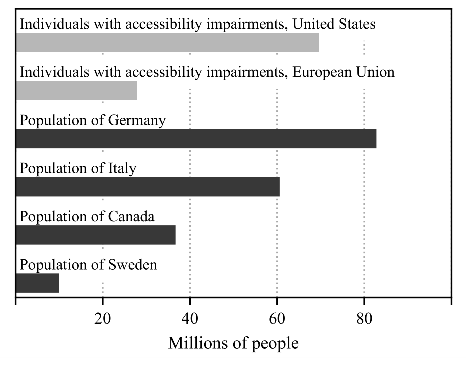
\includegraphics[width=0.88\columnwidth,height=5.0cm]{figures/population-plot}
    %% \hspace{1cm}
    %\caption{Number of people with software-related disabilities (e.g., vision, hand control, cognitive, or hearing) in the United States
    %and the European Union. 
    %% To put the numbers in perspective, the number of people with impairments is
    %% comparable to the population of entire countries. 
    %(Data compiled from: \cite{stats:accessibility_population:US, stats:accessibility_population:EU})}
    %\label{fig:population-plot}
  %% \end{figure}
  %\end{minipage}
  %\hspace{1cm}
  %\begin{minipage}[t]{.44\textwidth}
  %% \hfill
  %% \begin{figure}[b]
    %\centering
    %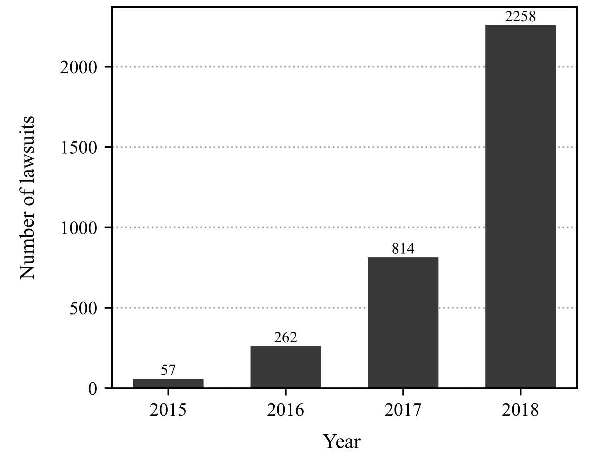
\includegraphics[width=0.91\columnwidth,height=5.0cm]{figures/lawsuits-plot}
    %\caption{Number of software accessibility lawsuits filed in US federal courts per year. The number of lawsuits increased by around 3800\% over the four-year period 2015-2018. (Data compiled from: \cite{stats:accessibility_lawsuits:US_1, stats:accessibility_lawsuits:US_2})}
    %\label{fig:lawsuits-plot}
  %% \end{figure}
  %\end{minipage}
  %\end{figure*}

\begin{figure}
    \noindent
	\begin{minipage}[c]{.97\columnwidth}
        \centering
        \begin{lstlisting}[language={HTML5},frame=ltbr,aboveskip=1.1em,basicstyle={\linespread{1.0}\footnotesize\ttfamily},]
<form>
<section>
 <div><p>Name</p></div>
 <div><p>Business Email</p><span>free providers not accepted</span></div>
</section>
<input type="text" id="vr_9481">
<textarea id="bx_3978"></textarea>
<input type="text" id="vr_6588">
<div><p>Message</p></div>
<section>
 <div><p>Do you have an open ticket?</p></div>
 <div><p>How often should we email you?</p></div>
 <span>Yes</span><span>No</span>
</section>
<input type="radio" value="Y" id="op_y">
<input type="radio" value="N" id="op_n" checked>
<select id="frq"><option>daily</option>
 <option>weekly</option><option>monthly</option>
</select>
</form>
        \end{lstlisting}
    (a) Sample of the HTML markup
    \end{minipage} \hfill
	\begin{minipage}[c]{\columnwidth}
        \centering
        \fbox{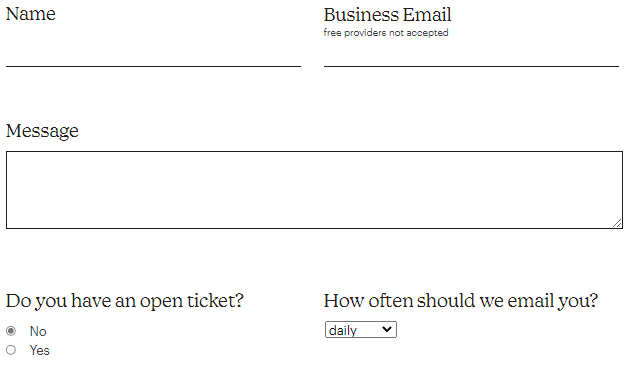
\includegraphics[width=\linewidth]{accessibility_repair/figures/motivating-example/rendered.png}}
        (b) Rendered form
    \end{minipage}
%	\begin{minipage}[c]{.98\columnwidth}
%	\centering \ \\
%	(a) Sample of the HTML markup
%	\end{minipage}
%	\begin{minipage}[c]{.98\columnwidth}
%	\centering \ \\
%	(b) Rendered form
%	\end{minipage}
	\ \\ \caption{An example of an inaccessible web form.}
    \label{fig:motivating-example}
  \end{figure}

This chapter makes the following main contributions:
\begin{itemize}
    \item A novel web form analysis approach for automatically inferring form 
    labeling markup, which is the first to address this issue, to the best of our knowledge.
    \item A technique that is based on a combination of visual cues and 
	optimization formulation to repair the DOM of a web form in order to have accessible labels. 
    \item A qualitative and quantitative evaluation in terms of accuracy, safety, and performance. 
The results show an average F-measure of 88.4\% for labeling accuracy, and an average run-time of around 1.6 seconds.
	\item An implementation of our approach, available in a tool called \toolname~\cite{tool-and-data}.
\end{itemize}

